\section{Caution}\label{caution}

For ground-contact surfaces in EnergyPlus, it is important to specify appropriate ground temperatures. Do not use the ``undisturbed'' ground temperatures from the weather data. These values are too extreme for the soil under a conditioned building. For best results, use the Slab or Basement program described in this section to calculate custom monthly average ground temperatures. This is especially important for residential applications and very small buildings. If one of these ground temperature preprocessors is not used, for typical commercial buildings in the USA, a reasonable default value is 2C less than the average indoor space temperature.

\section{Introduction}\label{introduction-003}

There are two difficulties behind linking ground heat transfer calculations to EnergyPlus. One is the fact that the conduction calculations in EnergyPlus (and in DOE-2 and BLAST previously) are one-dimensional and the ground heat transfer calculations are two or three-dimensional. This causes severe modeling problems irrespective of the methods being used for the ground heat transfer calculation. The other difficulty is the markedly different time scales involved in the processes. Basically, the zone model is on an hour scale and the ground heat transfer is on a monthly time scale. The basic heat balance based zone model of EnergyPlus has to be considered as the foundation for building energy simulation at the present time and for some time in the future. Thus, it is necessary to be able to relate ground heat transfer calculations to that model.

The heat balance zone model considers a single room or thermal zone in a building and performs a heat balance on it. A fundamental modeling assumption is that the faces of the enclosure are isothermal planes. A ground heat transfer calculation usually considers an entire building and the earth that surrounds it, resulting in non-isothermal face planes where there is ground contact. While it is not impossible to imagine multi-zone, whole building models that include the surrounding earth and non-isothermal building surfaces, such models will not be practical for some time in the future, and their usefulness even then is not clear.

The EnergyPlus development team addressed the problem and decided that the most reasonable first step would be to partially decouple the ground heat transfer calculation from the thermal zone calculation. The most important parameter for the zone calculation is the outside face temperature of the building surface that is in contact with the ground. Thus this becomes a reasonable ``separation plane'' for the two calculations. It was further decided that the current usage of monthly average ground temperature was reasonable for this separation plane temperature as well, since the time scales of the building heat transfer processes are so much shorter than those of the ground heat transfer processes.

Using the separation plane premise, the 3D ground heat transfer programs for slabs developed by Bahnfleth (1989, 1990) were modified by Clements (2004) to produce outside face temperatures. EnergyPlus permits separate monthly average inside temperatures as input. The program produces outside face temperatures for the core area and the perimeter area of the slab. It is described in the section ``Use of the Ground Temperatures with Slabs'' below.

A 3D basement program also is included with EnergyPlus. This is described below in Using Ground Temperatures with Basements. It uses the same principle as the slab procedure; it determines the outside face (surface) temperature of the walls and floor of a basement in contact with the ground.

It should be noted that either for slabs or basements the ground heat transfer is usually small unless the building is very small or has some special characteristics.

Multiple Ground Temperatures shows how the OtherSideCoefficients object of EnergyPlus can be used to supply multiple ground temperatures.

\section{Use of the Ground Temperatures with Slabs}\label{use-of-the-ground-temperatures-with-slabs}

The Slab program produces temperature profiles for the outside surface at the core and at the perimeter of the slab. It also produces the average based on the perimeter and core areas used in the calculation. This allows the user to apply the Slab temperatures one of two ways in EnergyPlus:

\emph{Option 1 - Core and Perimeter Temperatures}: The EnergyPlus OtherSideCoefficients object can be used to provide two sets of twelve monthly average ground temperature values. In this way, both the perimeter and the core values from the Slab program can be used in the succeeding EnergyPlus run. This method assumes that the floor slab will be described using at least two different heat transfer surfaces. The use of OtherSideCoefficients to provide additional ground contact surfaces is described in detail in the ``Multiple Ground Temperatures'' section below.

\emph{Option 2 - Average Temperatures:} Use the monthly average temperatures produced by the Slab program in the EnergyPlus GroundTemperatures object. This will provide an average ground temperature at the outside face of any heat transfer surface whose OutsideFaceEnvironment field is set to ``ground''.

EnergyPlus accepts twelve separate monthly average inside temperatures. In addition, it is possible to add an hourly sinusoidal variation of the inside temperature with a 24 hour period sine function. This was included to show the effect of something such as night setback on the face temperature. Generally, the effect is quite small.

First the results for a monthly specified constant average inside temperature. The location is Minneapolis, and the slab is insulated.

\begin{lstlisting}
Monthly Slab Outside Face Temperatures, C
Perimeter Area: 304.00  Core Area: 1296.00
Month   Average   Perimeter    Core      Inside
1      17.67     16.11      18.03       18.0
2      17.45     15.92      17.81       18.0
3      17.43     16.07      17.74       18.0
4      19.00     17.82      19.27       20.0
5      19.24     18.23      19.48       20.0
6      19.31     18.42      19.52       20.0
7      20.92     20.14      21.11       22.0
8      21.17     20.44      21.35       22.0
9      21.22     20.45      21.40       22.0
10      21.21     20.26      21.44       22.0
11      19.62     18.54      19.88       20.0
12      19.35     17.99      19.67       20.0
\end{lstlisting}

The resulting heat flux is shown below. The inside heat transfer coefficient and slab thermal properties are specified in the input file. For this example the total thermal resistance from the inside air to the slab bottom surface was 0.27 (m\(^{2}\) C)/W. This value is controlled by the user with the inside heat transfer coefficient and slab thermal properties values in the slab program input file.

\begin{longtable}[c]{p{0.85in}p{0.85in}p{0.85in}p{0.85in}p{0.85in}p{0.85in}p{0.85in}}
\toprule 
Month & Average & Perimeter & Core & Inside & Perimeter Heat Flux W/m & Average Heat Flux W/m \tabularnewline
\midrule
\endfirsthead

\toprule 
Month & Average & Perimeter & Core & Inside & Perimeter Heat Flux W/m & Average Heat Flux W/m \tabularnewline
\midrule
\endhead

1 & 17.67 & 16.11 & 18.03 & 18 & 7.00 & 1.22 \tabularnewline
2 & 17.45 & 15.92 & 17.81 & 18 & 7.70 & 2.04 \tabularnewline
3 & 17.43 & 16.07 & 17.74 & 18 & 7.15 & 2.11 \tabularnewline
4 & 19 & 17.82 & 19.27 & 20 & 8.07 & 3.70 \tabularnewline
5 & 19.24 & 18.23 & 19.48 & 20 & 6.56 & 2.81 \tabularnewline
6 & 19.31 & 18.42 & 19.52 & 20 & 5.85 & 2.56 \tabularnewline
7 & 20.92 & 20.14 & 21.11 & 22 & 6.89 & 4.00 \tabularnewline
8 & 21.17 & 20.44 & 21.35 & 22 & 5.78 & 3.07 \tabularnewline
9 & 21.22 & 20.45 & 21.4 & 22 & 5.74 & 2.89 \tabularnewline
10 & 21.21 & 20.26 & 21.44 & 22 & 6.44 & 2.93 \tabularnewline
11 & 19.62 & 18.54 & 19.88 & 20 & 5.41 & 1.41 \tabularnewline
12 & 19.35 & 17.99 & 19.67 & 20 & 7.44 & 2.41 \tabularnewline
\bottomrule
\end{longtable}

Then for the same conditions, the results with a 2 degree C amplitude 24-hour sine wave variation. Notice that the inside temperatures are the same since they are monthly averages and the daily variation oscillates about the mean. The core and perimeter slab temperatures are affected slightly.

\begin{lstlisting}
Monthly Slab Outside Face Temperatures, C
Perimeter Area: 304.00  Core Area: 1296.00
Month   Average   Perimeter    Core      Inside
1      17.51     16.03      17.86       18.0
2      17.29     15.85      17.63       18.0
3      17.27     16.00      17.57       18.0
4      18.87     17.77      19.13       20.0
5      19.11     18.16      19.34       20.0
6      19.17     18.34      19.37       20.0
7      20.81     20.07      20.98       22.0
8      21.05     20.36      21.21       22.0
9      21.09     20.38      21.26       22.0
10      21.08     20.19      21.29       22.0
11      19.47     18.45      19.71       20.0
12      19.20     17.92      19.51       20.0
\end{lstlisting}

An example of a 24-hour inside temperature profile for this case is shown below. The sine wave amplitude was 2 C.

\begin{lstlisting}
Day       Hour   Perim Out Ts    Core Out Ts    Inside Temp
1           1   17.30827       19.15832       18.51749
1           2   17.29503       19.15274       18.99974
1           3   17.30236       19.16732       19.41389
1           4   17.32258       19.19376       19.73175
1           5   17.34834       19.22526       19.93166
1           6   17.37288       19.25529       20.00000
1           7   17.39023       19.27798       19.93212
1           8   17.39544       19.28838       19.73265
1           9   17.38485       19.28117       19.41517
1          10   17.35602       19.24733       19.00130
1          11   17.30590       19.18686       18.51924
1          12   17.23507       19.10210       18.00180
1          13   17.14650       18.99703       17.48425
1          14   17.04291       18.87713       17.00183
1          15   16.92873       18.74895       16.58738
1          16   16.81076       18.61963       16.26915
1          17   16.69609       18.49656       16.06881
1          18   16.59243       18.38671       16.00000
1          19   16.50669       18.29626       16.06741
1          20   16.44276       18.23010       16.26645
1          21   16.40369       18.19161       16.58356
1          22   16.38873       18.18218       16.99714
1          23   16.39435       18.19834       17.47902
1          24   16.41942       18.23298       17.99639
\end{lstlisting}

A plot of the daily profiles is shown below. Note that the inside temperature change of 4 C produces only a small change in the slab lower face temperature.

\begin{figure}[hbtp] % fig 19
\centering
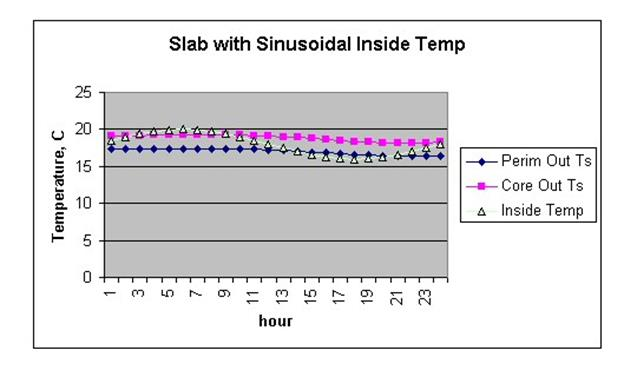
\includegraphics[width=0.9\textwidth, height=0.9\textheight, keepaspectratio=true]{media/image017.jpg}
\caption{Daily Temperature Profiles (Slab) \protect \label{fig:daily-temperature-profiles-slab}}
\end{figure}

The resulting heat fluxes are shown below. They can be compared with the fluxes shown above for the constant inside temperature run. The changes resulting from a fairly large 4 C daily temperature variation are probably not significant.

\begin{longtable}[c]{p{0.85in}p{0.85in}p{0.85in}p{0.85in}p{0.85in}p{0.85in}p{0.85in}}
\toprule 
Month & Average & Perimeter & Core & Inside & Perimeter Heat Flux W/m & Average Heat Flux W/m \tabularnewline
\midrule
\endfirsthead

\toprule 
Month & Average & Perimeter & Core & Inside & Perimeter Heat Flux W/m & Average Heat Flux W/m \tabularnewline
\midrule
\endhead

1 & 17.51 & 16.03 & 17.86 & 18 & 7.30 & 1.81 \tabularnewline
2 & 17.29 & 15.85 & 17.63 & 18 & 7.96 & 2.63 \tabularnewline
3 & 17.27 & 16 & 17.57 & 18 & 7.41 & 2.70 \tabularnewline
4 & 18.87 & 17.77 & 19.13 & 20 & 8.26 & 4.19 \tabularnewline
5 & 19.11 & 18.16 & 19.34 & 20 & 6.81 & 3.30 \tabularnewline
6 & 19.17 & 18.34 & 19.37 & 20 & 6.15 & 3.07 \tabularnewline
7 & 20.81 & 20.07 & 20.98 & 22 & 7.15 & 4.41 \tabularnewline
8 & 21.05 & 20.36 & 21.21 & 22 & 6.07 & 3.52 \tabularnewline
9 & 21.09 & 20.38 & 21.26 & 22 & 6.00 & 3.37 \tabularnewline
10 & 21.08 & 20.19 & 21.29 & 22 & 6.70 & 3.41 \tabularnewline
11 & 19.47 & 18.45 & 19.71 & 20 & 5.74 & 1.96 \tabularnewline
12 & 19.2 & 17.92 & 19.51 & 20 & 7.70 & 2.96 \tabularnewline
\bottomrule
\end{longtable}
